% Sidst opdateret: 25/1 1994
\documentstyle[a4,nfdcfnt,12pt]{article}
\input{psfig}
\parindent=0cm
\pagestyle{empty}
\begin{document}
\Large
\vspace{5cm}
\begin{center}
Seminar about \\
The Kinetic Compiler \\

\vspace{2cm}
Kenneth Geisshirt \\
25 January 1994
\end{center}

\vspace{5cm}
\begin{itemize}
\item Chemical Kinetics.
\item Motivation.
\item The Basic Components.
\item Overall Structure of Input.
\item Reactions and Ordinary Differential Equations.
\item Simulations.
\item A Larger Example.
\end{itemize}
\newpage

\begin{center}
Chemical Kinetics
\end{center}

\vspace{2cm}
The chemical kinetics (in a stirred system) is modeled by

\[
  \frac{d\vec{c}}{dt} = \vec{f}(\vec{c}),
\]

\vspace{1cm}
and with diffusion

\[
  \frac{\partial\vec{c}}{dt} = \vec{f}(\vec{c}) + \mathbf{D}\nabla^2 \vec{c}.
\]

\vspace{1.5cm}
From the velocity of each reaction, one can write

\[
  \frac{d\vec{c}}{dt} = \mathbf{\nu}\vec{v}(\vec{c}).
\]

\newpage
\begin{center}
Motivation
\end{center}

\vspace{1cm}
The law of mass action gives us the velocity

\[
  v_i = k_i \prod_{j=1}^r c_j^{\nu_{ij}}.
\]

With $r\approx 10$ and $n\approx 10$ the complexity is high, i.e.\ easy
to make an error.

\vspace{2cm}
The real motivation is the complexity of the Jacobian

\[
  J_{ij} = \frac{df_i}{dc_j}.
\]

In the numerical solution, the Jacobian is needed, because of the stiffness
of the equations. 

One could use numerical differentiation

\[
  \frac{df_i}{dc_j} \approx \frac{f_i(c_j+h)-f_i(c_j-h)}{2h},
\]
but it gives poor results.

For example Calahan's method:

\begin{eqnarray*}
\vec{k}_r &=& T({\mathbf E} - Ta_1 {\mathbf J}(\vec{c}_r))^{-1}\vec{f}(\vec{c}_{r-1}) \\
\vec{l}_r &=& T({\mathbf E} - Ta_1 {\mathbf J}(\vec{c}_r))^{-1}\vec{f}(\vec{c}_{r-1}+b_1\vec{k}_r) \\
\vec{c}_r &=& \vec{c}_{r-1} + R_1\vec{k}_r + R_2\vec{l}_r
\end{eqnarray*}

\newpage
\begin{center}
The Basic Components
\end{center}

\vspace{1cm}
\begin{description}
  \item[Numbers] Legal numbers are:\\
    10 \\
    3.14 \\
    3.0e-6 \\
    4.4L+10
  \item[Names] A name is a letter followed by letters and/or numbers. E.g.\ \\
    HelloWorld \\
    pi \\
    Pi \\
    Const1b 
  \item[Species] Legal species are: \\
    H2O \\
    so4(-2) \\
    H(+) 
  \item[Concentrations] are species in brackets: \\
    {\rm [}H2O{\rm ]} \\
    {\rm [}so4(-2){\rm ]} \\
    {\rm [}H(+){\rm ]}
\end{description}

\newpage
Expressions are typed as in ordinary programming languages. In general:

\vspace{.5cm}
expr op expr \\
- expr \\
( expr ) \\
func ( expr )

\vspace{.5cm}
Operators (op) are +, -, *, /, **, and functions (func) can be
the standard functions. 

\vspace{.5cm}
Legal expressions are:

2+x;\\
4-(x**1.5)-(x+y)/2;\\
3+exp(x)*sin(t);

\newpage
\begin{center}
General Structure of an Input File
\end{center}

\psfig{file=struct.ps,width=14cm,height=15cm}

\vspace{2cm}
Declaration of constants:\\
time = 2.50;
 
\newpage
\begin{center}
Reactions and Ordinary Differential equations
\end{center}

A reaction is written in the form:

number: coeff spec + $\cdots$ -> coeff spec + $\cdots$; k>=expr;

\vspace{.5cm}
Examples of legal reactions:

20: A + 2B -> C; k>=2.0;\\
42: A(+) + B <-> 2B; k>=2.0; k<=4.1;\\
45: A -> B + C; v>=[A]/(1+2*[B]*[C]\ $\hat{}$\ 3);\\
63: B <-> A; v>=[A]/[B]\ $\hat{}$\ 2; k<=2.12;

\vspace{3cm}
Ordinary differential equations can be used as well. 

They are written in the form:

\vspace{.25cm}
name' = expr;

\vspace{.5cm}
Legal differential equations are:

x' = x;\\
temp' = sin(t)*exp(temp-2*kb*[A]);

\newpage
\begin{center}
Constraints and Initial Values
\end{center}

\vspace{1cm}
In chemical kinetics one often has constraints in the form

\[
  \sum_{i} [S_i] = C.
\]

If one rewrites them to

\[
  [S_{i\prime}] = C - \sum_{i\not =i\prime} [S_i],
\]

{\tt kc} is able to use them. For example:

\[
  [{\mathrm Ce^{4+}}] + [{\mathrm Ce^{3+}}] = C_{\mathrm tot}
\]

is written as \\
{\rm [}Ce($+4$){\rm ]} = Ctot - {\rm [}Ce($+3$){\rm ]};

Actually, the right hand side can be any expression.

\vspace{2cm}
Concentrations and dynamical values can be assigned a value
at $t=0$. For example:\\

[A](0) = 1.2e-10;\\
temp(0) = 273.15;

\newpage
\begin{center}
Making Simulations
\end{center}

\vspace{1cm}
To simulate a CSTR one has to go through two steps.

\begin{itemize}
\item Write a input file;
\item Run the simulation program: {\tt kkin file-name}.
\end{itemize}

The output file is {\tt kinwrk.dat} and is in GNUplot format.
\end{document}
